\chapter{Webauftritt}
\renewcommand{\kapitelautor}{Autor: Hatice Akyokus}
In diesem Kapitel wird der Webauftritt erläutert. Der Webauftritt ist der wichtigste Bestandteil der Diplomarbeit, da sich alle Elemente auf dieser befinden.
 
\section{Intention}
Um die Zielgruppe am Besten zu erreichen, wurde eine Webseite erstellt. In dem Zeitalter des Internets, ist es sehr wichtig, den Webauftritt auf eine kreative Art und Weise zu gestalten. Vor allem, da diese Diplomarbeiten Informationen über die Medientechnik vermitteln möchte. Eine Informationsseite, welche aufzählt, was an der HTL Rennweg beigebracht wird, wäre langweilig und würde die Zielgruppe nicht erreichen. Aus diesem Grund, wurden viele Brainstormings durchgeführt, um die beste Vorangehensweise zu ermitteln. Die große Schwierigkeit hierbei war es, die Webseite an die Zielgruppe anzupassen, da sie die Medientechnik nicht kennen. Daher mussten alle Erklärungen und technische Aspekte, so einfach wie möglich erklärt werden, um sie nicht zu verschrecken. Durch die Problematik am Tag der offenen Tür, soll die Webseite auch Missverständnisse beseitigen und dafür sorgen, dass User, eine Entscheidung treffen können, die sie später nicht bereuen. 

\section{Inhalt}
Die Entscheidung, welche Inhalte auf der Webseite zu sehen sind, war nicht leicht, da die Medientechnik ein sehr großer Bereich ist. Sehr früh hat sich das Team darauf geeinigt, die Medientechnik mit der Größe des Universums zu vergleichen und die Webseite in einem „Space-Theme“ zu halten. Wie bei jedem Webauftritt üblich, enthält diese eine Startseite, welche einen Vorgeschmack geben soll und weitere Informationen bietet. Informationen über die Medientechnik findet sich in zehn Lektionen, welche das Team aufbereitet hat und zeigt, was in den fünf Jahren Medientechnik beigebracht wird. Da sich der Lehrplan allerdings ändern wird, wurden die Lektionen allgemein gehalten und bieten einen Einblick in die Basics der Mediengestaltung, Animationen und Spiele. Um die Informationen spannender zu präsentieren, wurden interaktive Elemente hinzugefügt, welche die User für die Medientechnik begeistern sollen. Da Videos auch eine wichtige Rolle in der Medientechnik spielen, wurden Interviews und auch ein Animationsvideo gedreht, welche es als Ziel hatten, die User über die Schule im Allgemeinen und die Medientechnik zu informieren. Durch diese ganzen Elemente soll gewährleistet werden, dass die User über die HTL Rennweg informiert sind und eine Entscheidung treffen können. 

\section{Hosting}
Webhosting stellt Speicherplatz in Internet bereit. Für dies ist ein leistungsstarker Rechner notwendig. Um die Inhalte jederzeit abrufen zu können, ist deshalb eine Internetverbindung notwendig. Je nach Anbieter und Angebot, ändert sich der Leistungsumfang im Webhosting.   Das Team entschied sich anfangs für das Webhosting durch easyname.at, weil es ein Jahr lang kostenlos ist und viel Speicherplatz zur Verfügung stellt. Allerdings hat sich nach kurzer Zeit herausgestellt, dass die Leistung nicht den Wünschen des Teams entsprach und somit musste, die Domain, welche im Angebot enthalten war, transferiert werden. Nach einer langen Suche, nach einem geeigneten Webhoster, stieß das Diplomarbeitsteam auf syhost.at, welche auch ein Angebot bietet, welches ein Jahr lang kostenfrei ist. Einzig die Kosten für die Domaintransferierung mussten bezahlt werden. Die Leistung von syhost.at, entsprach mehr den Vorstellungen des Teams. Mittels dem File Transfer Protocol Client „Filezilla“, werden die Webseiten hochgeladen und den Usern zur Verfügung gestellt. 



\section{Bildquellen}
Alle verwendeten Bilder, wurden von der Webseite unsplash.com heruntergeladen. Unsplash.com ist eine Webseite, auf der User Bilder, die sie selbst geschossen haben, hochladen können. Diese können von anderen Usern kostenlos heruntergeladen werden. Weiters wurden kostenlose Vektorgrafiken von der Webseite flaticon.com verwendet. Dies ist eine Webseite, welches Vektorgrafiken in verschiedenen Formaten anbietet. Es gibt kostenpflichtige und kostenfreie Grafiken, die frei anpassbar sind. Für die Webseite wurden kostenfreie Vektorgrafiken verwendet. Im Rahmen der Diplomarbeit wurden Bilder verwendet, die dem Corporate Design entsprechen und zu dem Thema der Diplomarbeit passen. Das Team entschied sich für ein „Space-Theme“, welches die Größe der Medientechnik grafisch darstellen sollte. 

\section[Frameworks und Libraries]{Frameworks und Libraries\protect\footnote{\label{foot:2}vgl.https://www.eins2design.de/blog/168-was-bedeutet-framework-und-wozu-wird-es-verwendet [Zugriff: 18.03.2018]}} 
Framework heißt übersetzt Rahmenkonstruktion und wird häufig bei Webseiten verwendet. Sie dienen als Gerüst zum Programmieren und erleichtern die Arbeit, die damit verbunden ist. Dabei ist das Framework selbst kein Programm, sondern ein Rahmen, welcher den Inhalt ansprechend präsentiert. 

\subsection{Content Delivery Network}
Ein Content Delivery Network sorgt für eine schnelle und zuverlässige Auslieferung von Medieninhalten, welche mit Hilfe von Caching im Internet vorgehalten werden. 

\begin{quote}
Das CDN besteht aus einem Ursprungsserver (Originserver), auf dem die zu verteilenden Inhalte ablegt werden, vielen Replica-Servern, welche die Kopien der Inhalte vorhalten, sowie einem Distributionssystem, das die Inhalte auf den Replica-Servern verteilt. Für die Umleitung der Nutzeranfragen auf die einzelnen Replica-Server sorgt ein Request-Routing-System. Nachdem ein Client eine Anfrage an das Content Delivery Network gesendet hat, wählt das Request-Routing-System den geeigneten Replica-Server aus. Bei der Auswahl bezieht es Kennzahlen über deren aktuelle Belastung (CPU-Auslastung, Menge der aktiven Verbindungen etc.) und über die Netzwerkverbindung zwischen dem anfragenden System und dem Server mit ein. Ist der Server ausgewählt, wird die Nutzeranfrageentsprechend umgeleitet.
\end{quote}

Die Vorteile eines Content Delivery Networks sind die schnellen Ladezeiten, die hohe Ausfallsicherheit und eine optimale globale Lastverteilung.   Allerdings kann man die Dokumente, welche man von einem Content Delivery Network bezieht, nicht optimieren. Vor allem bei CSS-Frameworks ist dies ein großer Nachteil, weil man die CSS-Styles überschreiben muss. Außerdem gibt es keine Garantie, dass die Webseite pre-cached wurde, da vor allem mobile Geräte einen kleinen und ineffizienten Cache haben. Ein wichtiger Punkt ist, dass Content Delivery Networks nicht in allen Ländern zur Verfügung stehen, da Sie aus geografischen oder politischen Gründen blockiert werden. Allerdings ist dies kein Problem für die Diplomarbeit Insight, weil die Webseite nur für User in Österreich gedacht ist.  
\\
Da FontAwesome verwendet wurde, welche eine große Datei zum Herunterladen ist, entschied sich das Team dazu ein Content Delivery Network zu verwenden. 
\\
Das CSS-Framework Foundation und alle anderen Javascript-Frameworks wurden heruntergeladen und deren CSS beziehungsweise Javascript Dokumente eingebunden. Dies hat den Vorteil, dass man die CSS und Javascript Dokumente nach Belieben optimieren kann. Somit hat man mehr Kontrolle über das Framework. Weiters spielt die Internetgeschwindigkeit eine große Rolle. Die Webseite wird, wenn das Framework lokal gespeichert ist, schneller geladen bei einem schlechten Internetzugang. 

\subsection{CSS-Frameworks} 
Ein CSS-Framework, sorgt für das Layout der Webseite. Da sie die meiste Programmierarbeit wegnimmt, kann man produktiver arbeiten und Fehler vermeiden. Weiters, hat man einen besseren Workflow im Team und eine optimale Browser-Kompatibilität. 
Ein solches Framework beinhaltet vordefinierte CSS-Klassen, welche einfach zu benutzen sind, typographische Style Definitionen und ein Grid System.  
Allerdings braucht man mehr Zeit, um das Framework zu verstehen. Deswegen ist es sehr wichtig, dass das Framework eine sehr gute Dokumentation hat, welche gut gepflegt wird. Größere CSS-Frameworks bieten auch Javascript-Files, welche erweiterte Funktionen bieten. Im Rahmen der Diplomarbeit wurde das CSS-Framework Foundation verwendet.

\subsubsection{Bootstrap oder Foundation}
Das CSS-Framework Foundation hat eine kleine Community, somit sind die Foren eher leer und bieten nicht mehrere Antworten für eine Frage. Die Dokumentation ist zwar gut, aber manche Fehler konnten auch mit dieser nicht gelöst werden. Deswegen überlegte sich das Team in dem Anfangsstadium der Diplomarbeit auf das CSS-Framework Bootstrap umzusteigen. Um eine geeignete Entscheidung treffen zu können, wurden beide Frameworks verglichen. Bootstrap ist um einiges beliebter als Foundation und hat eine größere Community. Genauso, wie Foundation basiert Bootstrap auch auf einem Grid-System. Während Bootstrap auf einem Flex-Grid basiert, bietet Foundation mehrere Möglichkeiten an Grids an. Es gibt ein XY Grid, welches horizontal oder vertikal angelegt werden kann. Außerdem kann man der Grid noch weitere Eigenschaften zuweisen.   Weiters hat Foundation eine Topbar, welche eine Navigationsleiste ist, welche sich mehr auf die Struktur konzentriert als auf das Design, was bedeutet, dass man die Navigationsleiste individuell designen muss. Dies ist ein Vor- und Nachteil, da die Navigationsleiste individuell gestaltbar ist und nicht zwingend wie andere Navigationsleisten aussieht aber dahinter steckt wiederrum Programmierarbeit, was bei Bootstrap nicht der Fall ist. Doch die Navigationen von Webseiten, die mit dem Framework Bootstrap entwickelt wurden, haben ein für Bootstrap typisches Styling.   Allerdings hat Bootstrap in Sachen wie den Support für mobile Geräte die Nase vorne. Weiters bietet sie sehr viele Templates, welche sehr beliebt sind. Bootstrap konzentriert sich, wie bereits erwähnt, mehr auf das Design und Foundation hingegen legt sehr viel Wert auf Responsiveness und Funktionalitäten. Für Anfänger wird Bootstrap empfohlen. Das Team entschied sich im Endeffekt für Foundation, da es eine neue Herausforderung für das Team ist und Foundation einen fluiden Ansatz bietet und mehrere Funktionen bietet als Bootstrap. 


\paragraph{Foundation}
Foundation ist ein CSS-Framework und wirbt damit, für jedes Gerät geeignet zu sein. Es sorgt für Responsiveness und Einfachheit beim Designen der Webseite. Foundation basiert auf dem Mobile First Prinzip, was bedeutet, dass die Darstellung auf mobilen Endgeräten die höchste Priorität hat.   Außerdem bietet das Framework die Möglichkeit, alle Elemente nach Belieben zu ändern. Mit ihren vordefinierten Klassen, sorgt das Framework für einen sauberen und effizienten Code, welcher im optimalsten Fall leicht zu verstehen ist. Die einzige Herausforderung war es, sich in das Framework einzuarbeiten, welches ein bisschen Zeit beanspruchte. 

\paragraph{Slick Slider}\\
Slick Slider ist ein Framework, welche hauptsächlich für Slider gedacht ist. Da die Webseite dieser Diplomarbeit auf diesem Prinzip beruht, entschied sich das Team dazu, Slick Slider zu verwenden. Der Entwickler dieses Frameworks wirbt für Slick mit folgendem Slogan: „Slick – the last carousel you’ll ever need“ . Slick ist sehr einfach zu bedienen, da die Programmierarbeit sehr minimal ist. Die nötigen Methoden werden bereits vom Framework angeboten, wobei man sehr viel anpassen kann. Somit muss man die vordefinierten Klassen nicht verwenden und kann es vom Aufbau her, so gestalten wie man möchte. Dies wurde in der Diplomarbeit natürlich ausgenutzt um die Webseite einzigartig erscheinen zu lassen. Slick bietet dem Nutzer sehr viele Möglichkeiten an, die Slider zu steuern oder zu gestalten und ist responsive und basiert ebenfalls auf dem mobile-first Prinzip. Außerdem bietet Slick den Nutzern die Möglichkeit, Breakpoints zu setzen.

\begin{figure}[H] 
  \centering
     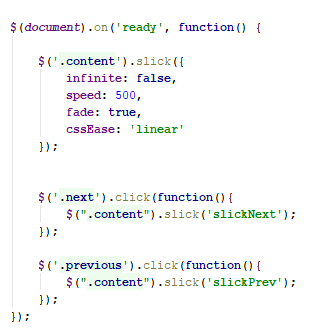
\includegraphics[width=0.7\textwidth]{webseite_abb1.png}
  \caption{Aufruf von Slick Slider}

\end{figure}

Wie man in der Abbildung sehen kann, wird Slick aufgerufen. Es können vordefinierte Parameter übergeben werden, welche man nach Belieben einstellen kann. Das Team hat außerdem eigene Buttons zum Weiterschalten definiert, welche sich nicht, wie bei Sliders üblich, links und rechts befinden, sondern unterhalb. Slick wurde ebenfalls heruntergeladen und lokal hinzugefügt.

\paragraph{Create JS} \\
Create JS ist eine Sammlung von Libraries, welche entweder zusammen arbeiten oder individuell angewendet werden können. Diese Libraries basieren auf Javascript und bestehen aus:
\begin{itemize}
\item EaselJs
\item TweenJs
\item SoundJs
\item PreloadJs
\end{itemize}

EaselJS wurde für diese Diplomarbeit verwendet und ist dafür gedacht, dass man besser mit dem HTML 5 Canvas arbeiten kann. EaselJS wurde für die siebte Lektion verwendet. 

\paragraph{interact.js}\\ 
Interact.js ist ein Javascript-Framework, welches für Drag and Drop und Muti-Touch-Gesten gedacht ist. In der Diplomarbeit wird sie für das sechste Kapitel verwendet. 


\section{Responsiveness}
Responsive Webdesign bedeutet, dass sich der Inhalt einer Webseite an die Bildschirmauflösung des Endgeräts anpasst. Der steigende Marktanteil von Smartphones und Tablets zwingt die Entwicklung von responsiven Webseiten. Dabei soll die Trennung zwischen einer Mobil- und Desktopversion vermieden werden, da dadurch ein erhöhter Pflegeaufwand entsteht. Durch die stetige Änderung von Tablet- und Smartphoneformate, werden mehrere Versionen von Nöten sein und das soll mit einer responsiven Webseite verhindert werden. 
Um zu gewährleisten, dass die Webseite auf allen Endgeräten einwandfrei funktioniert, wurde auf eine responsive Webseite einen sehr großen Wert gelegt. Vor allem, da die Webseite sehr viele Bilder enthält.


\begin{quote}
Responsive Webdesign ist kein Trend! Studien zum Absatz mobiler Endgeräte belegen eine stetige Zunahme der Verkäufe von Tablets und Smartphones. Diese Entwicklung wird nicht nur von der Fachszene mit Euphorie verfolgt, es gibt auch fast täglich neue Entwicklungen zum Thema der technischen und grafischen Umsetzung von Webseiten für mobile Endgeräte. Responsive Webdesign spielt mit der geräteübergreifenden Flexibilität eine tragende Rolle in dieser Bewegung die sich zunehmend zu einem Standard entwickelt. 
\end{quote}

Durch Responsive Design wird eine bessere Bedienbarkeit gewährleistet und somit die Bounce-Rate deutlich reduziert. Außerdem ergibt sich weniger Wartungsaufwand bei Updates.  Das CSS-Framework hilft dabei als Gerüst, die Webseite responsiv zu machen. Allerdings muss auch nachgeholfen werden und dies erfolgte hauptsächlich mit Flexbox. Dies ist eine sehr einfache Möglichkeit, flexible Layouts zu erstellen, ohne CSS-Einstellungen wie position zu verwenden. In der Diplomarbeit wurde sie hauptsächlich dafür verwendet, Elemente zu zentrieren, denn dies erweist sich, vor allem für das vertikale Zentrieren von Elementen, als kompliziert. 

\begin{figure}[H] 
  \centering
     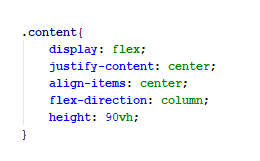
\includegraphics[width=0.7\textwidth]{webseite_abb2.png}
  \caption{Anwendung von Flexbox}

\end{figure}

Wie in der Abbildung zu erkennen ist, wird auf das Element mit der Klasse content, eine Flexbox angewendet. Alle Kindelemente von content werden, sowohl horizontal als auch vertikal zentriert angezeigt. Außerdem wurden bei den Größenangaben keine Werte in Pixel angegeben. Das Pixel ist eine absolute CSS Einheit und darin liegt auch das Problem, denn sobald die Webseite verkleinert wird, bewegt sich der Inhalt nicht mit und ist somit nicht responsiv. Deswegen wurden relative CSS Einheiten, wie vw, vh und rem verwendet. Die Einheiten vw und vh stehen für viewport width und viewport height und entsprechen dem 100. Teil der Breite des Anzeigebereiches. Allerdings werden sie vom Internet Explorer erst ab Version 9 unterstützt. Die Einheiten viewport width und viewport height wurden für Div-Boxen verwendet, da es wichtig ist, dass sie responsiv sind.  Für Schriftarten wurde rem, root em, verwendet. 

\begin{quote}
„rem verhält sich genauso wie em mit dem einzigen Unterschied, dass das sich der rem-Wert am Root-Element orientiert (also an der Schriftgröße, für body bzw. html), statt sich wie em an der Schriftgröße des jeweiligen Eltern-Elements zu orientieren.“
\end{quote}

Da rem nicht von älteren Browsern unterstützt wird, musste eine Fallback-Lösung in px im Stylesheet definiert werden.   Außerdem wurden Breakpoints eingearbeitet, um eine Responsiveness, vor allem für mobile Geräte, zu gewährleisten. 

\subsection{Startseite}
Die Startseite ist eine wichtige Seite, welche das Interesse anregen soll. Es war dem Team sehr wichtig, die Startseite so modern wie möglich zu gestalten, um den User dazu zu bringen die Webseite zu erkunden. Auf der Navigationsleiste befindet sich das Logo und weitere Links, über uns, Download, Kontakt und ein FAQ. Diese sind sehr simpel gehalten. Die Navigationsleiste ist schlicht gehalten und weiß. Die Schrift ist in dem orange des Corporate Designs und wenn man mit der Maus über die Links fährt, werden sie grün. 

\begin{figure}[H] 
  \centering
     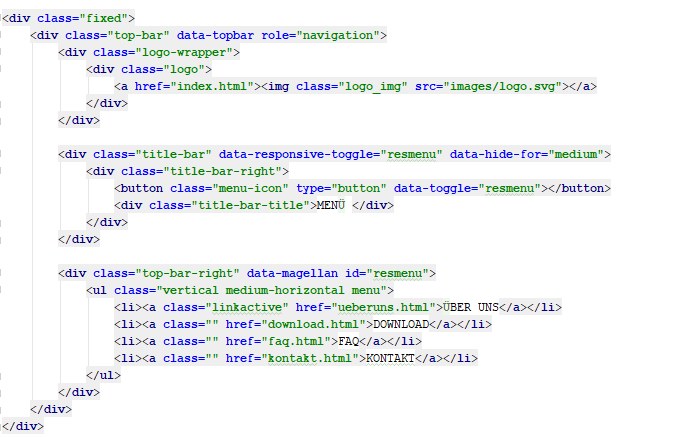
\includegraphics[width=0.7\textwidth]{webseite_abb3.png}
  \caption{Aufbau der Navigationsleiste}

\end{figure}

DDie Navigation besteht aus drei Containern, wobei eines das Logo enthält, eines welches bei Verkleinern des Bildschirms einen Burger Menü erscheinen lässt und eines, welche die Links zu den erwähnten Links enthält. Ein Burger Menü, ist ein Icon, welches beim Klick eine versteckte Navigation erscheinen lässt. Das ist vor allem bei mobilen Geräten sehr nützlich.  Die Klasse „linkactive“, hebt die Seite, auf der man sich gerade befindet, hervor. \\

Die Seite Über Uns, gibt dem User Informationen über die Entwickler der Webseite und den Nutzen den diese hat. Sie wurde entwickelt, um die User mit den Entwicklern vertraut zu machen. Sie ist, wie alle anderen Seiten, im Space-Theme gehalten. 
\\

Weiters kann man ein Dokument, welches zusätzliche Informationen über die Medientechnik enthält und zur Webseite ergänzend wirken soll, herunterladen. Dieses ist sehr detailliert und ist auch für die Eltern der Schüler gedacht, um soviel Informationen, wie möglich über die Medientechnik zu bekommen. 
\\
Bei Fragen, kann auf die Kontaktseite wechseln, welches ein Kontaktformular enthält, was das Kontaktieren der Schule vereinfachen soll. Außerdem befinden sich auf dieser Seite auch Kontaktinformationen der Schule, falls es User präferieren die HTL anzurufen.\\

Der User hat allerdings auch die Möglichkeit, in das FAQ (Frequently Asked Questions) einen Blick zu werfen, auf der sich häufig gestellte Fragen befinden. Somit entlastet man diejenige Person, die sich um die Fragen kümmert. Die Fragen wurden am Tag der offenen Tür gesammelt und auch selbst ausgedacht. 


\section[Storytelling]{Storytelling\protect\footnote{\label{foot:2}vgl. https://www.textbroker.de/storytelling [Zugriff: 18.03.2018]}}

\begin{quote}
Kinder verpacken Ihre Ideen und Gedanken oftmals in Geschichten, um uns Erwachsene damit ihre Welt zu erklären. Als Erwachsene wiederum müssen wir es wieder lernen, Geschichten zu erzählen.
\end{quote}
Storytelling vermittelt durch den Einsatz von Geschichten Information. Die Geschichten können real oder konstruiert sein, es muss lediglich gut ankommen und im Kopf der Nutzer bleiben. Weiters dient Storytelling dazu, die Aufmerksamkeit des Nutzers auf eine kreative Weise zu ergattern. Die Informationen werden dabei anschaulich gemacht, um die Botschaft ankommen zu lassen. Wichtig ist die Erstellung eines oder mehreren Protagonisten und einem Problem. Im Laufe der Geschichte, soll sich das Problem lösen aber das muss nicht unbedingt sein. Eine gute Geschichte führt dazu, dass sich die Nutzer mit der Thematik auseinandersetzen und emotional aufgeladen sind. Weiters sorgt eine gute Story für Begeisterung. Es gibt verschiedene Arten von Storytelling, vom Buch bis hin zu Werbevideos und Webseiten. Das Internet bietet hier eine große Möglichkeit für das Erzählen von Geschichten. Wichtig ist vor allem die Interaktivität, damit es nicht zu schnell langweilig wird.  Für das Team war es wichtig, die Zielgruppe durch die Geschichte zu erreichen. Dabei sollten Klischees vermieden werden und die Nutzer sollten sich mit dem Erzähler identifizieren können. 

\subsection{Story}
Project Insight benutzt klassische Storytelling-Methoden, um Nutzer über die Medientechnik zu informieren. Dabei dachte sich das Team, die Figur, Rene Weg, aus. Dieser ist ein Absolvent der HTL Rennweg und hat dem Nutzer gegenüber eine Mentor-Funktion. Rene Weg, ist eine sarkastische und humorvolle Figur, welcher dem Nutzer die Medientechnik, auf eine spielerische und lockere Art und Weise, präsentiert. Es war dem Team sehr wichtig, ein paar Witze in die Story einzubinden, um dem Nutzer das Gefühl zu geben, dass man an der HTL Rennweg auch Spaß haben kann. Durch verschiedenste Gestiken und Mimik, wird Leben in die Figur gehaucht. 

Abgesehen von der Rolle der Figur als Mentor, kommt sie auch noch in dem Animationsvideo (siehe Kapitel Animationsvideo) vor. 

\subsubsection{Aufbau}
Die Story ist in zehn Lektionen aufgeteilt. Dabei arbeitet sich der User stufenweise in die Medientechnik ein. Es beginnt mit einer Einführung und geht Schritt für Schritt die vorgegebenen Bereiche der Medientechnik durch und endet anschließend mit einem humorvollen Video. Bevor die Story beginnt, wird der User darauf hingewiesen, dass die Webseite Audio beinhaltet. Die Webseite wird vom Charakter, Rene Weg, vertont. 
Für das Grundgerüst wurde das Framework Slick Slider verwendet. Dabei wurde ein Grid erstellt, wo sich auf einer Seite der Text und auf der anderen Seite die Figur befindet. 
\\

Zusätzlich befinden sich unter dem Text vier Buttons, welche für das Weiterschalten und für das Pausieren und Abspielen gedacht sind. 


\begin{figure}[H] 
  \centering
     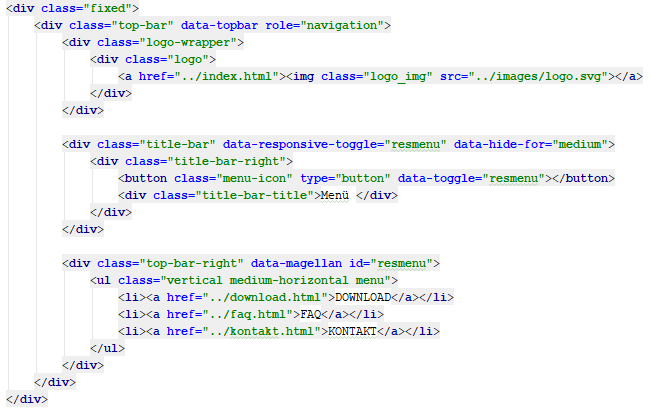
\includegraphics[width=0.7\textwidth]{webseite_abb4.png}
  \caption{Aufbau einer Slide}
  
  \centering
  	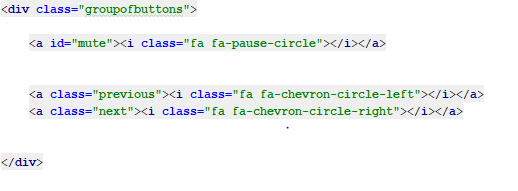
\includegraphics[width=0.7\textwidth]{webseite_abb5.png}
  \caption{Aufbau der Weiterschalt-Buttons}

\end{figure}

In den beiden Abbildungen ist die Struktur der Webseite zu sehen. Jedes Slide hat eine eigene ID und zwei Kindelemente, welche sich jeweils links und rechts befinden und den Text und die Figur beinhalten. Das Element mit der Klasse „groupofbuttons“ beinhaltet die Buttons mit denen man zum nächsten Slide gelangt. Klickt man auf die Next und Previous Buttons, kommt man zum nächsten Slide. Sobald man auf den Pause-Button klickt, wird das Audio pausiert und kann durch den Play-Button wieder abgespielt werden. Will man sich das Audio noch einmal anhören, so kann man ebenfalls auf den Play-Button klicken. Die große Problematik beim Aufbau war es, pro Slide ein einziges Audio-File abzuspielen. Öfters ist es vorgekommen, dass beim Weiterklicken, das vorherige Audio-File noch mitspielt. Um dies zu verhindern, wurden if-Statements eingebaut, welche überprüfen, ob sich der User in einem bestimmten Slide befinden. Befindet sich der User beispielsweise im zweiten Slide, wird das zugehörige Audio-File abgespielt. Sobald man das zweite Slide verlässt, pausiert sich das Audio-File, so dass sich keine Audio-Files überkreuzen. 

\\

Nicht jedes Slide hat ein Audio-File, da es Slides gibt, welche den User darüber informieren, welche Lektion gerade bearbeitet wird. Bei diesen Slides, ändert sich die Struktur, denn die Play und Pause-Buttons verschwinden und die Buttons zum Weiterschalten rücken in die Mitte. Außerdem gibt es Slides, welche Videos beinhalten und nicht vertont wurden, welche ebenfalls keine Play und Pause-Buttons enthalten. 

\\ 

Am Ende der Lektion, wurde dem Weiterschalt-Button ein Link zur nächsten Lektion hinzugefügt. 

 \\

Hierbei wird der letzte Slide ermittelt und dem Weiterschaltbutton ein Link hinzugefügt. Durch die im Bild abgebildete Methode, muss pro HTML-Dokument nur der Link zum nächsten HTML-Dokument angegeben werden. 

\\

In den folgenden Absätzen, werden alle Lektionen zusammengefasst.
\paragraph{Lektion 1}\\
In der ersten Lektion wird der Charakter, Rene Weg, vorgestellt. Nachdem sie sich humorvoll vorgestellt hat, werden Fragen rund um die HTL beantwortet. Um dies veranschaulichen zu können, wird ein Animationsvideo vorgeführt. Die erste Lektion dient nur als Einführung in eine HTL und soll die User mit Rene Weg bekannt machen. 


\paragraph{Lektion 2}\\
Da die HTL etwas Neues für die User ist und sie nicht wissen, was ein Abteilungsvorstand ist, geht es in der zweiten Lektion um ihn. Dabei wird erklärt was ein Abteilungsvorstand ist. Außerdem wird ein Interview mit dem Abteilungsvorstand der HTL Rennweg, Dr. Gerhard Hager, gezeigt. 

\paragraph{Lektion 3}\\
Wenn man im Internet nach der Medientechnik recherchiert, dann findet man komplexe Erklärungen, die sich teilweise widersprechen. Aus dem Grund, hat sich das Team dazu entschlossen in der dritten Lektion die Medientechnik zu erklären. Diese Lektion ist die einzige Lektion, in der es keine interaktiven Elemente gibt. Rene Weg vergleicht dabei die Größe der Medientechnik mit der des Universums und bezieht sich somit auf das „Space-Theme“. 

\paragraph{Lektion 4}\\
Mediengestaltung spielt eine große Rolle und wird in der vierten Lektion behandelt. Dabei erklärt Rene Weg dem User, wie wichtig es ist langweiligen Inhalt, spannend zu gestalten. Als Beispiel wird die Entstehungsgeschichte der HTL aufgelistet und danach wird eine spannendere Auflistung hergezeigt. Dieses Kapitel dient dazu, dem User zu zeigen, wie wichtig Kreativität in der Medientechnik ist und dass man mit seinem Inhalt hervorstechen muss, um erfolgreich zu sein.

\paragraph{Lektion 5}\\
Spiele sind sehr populär und werden in der fünften Lektion behandelt. Viele Interessenten, interessieren sich für die Entwicklung von Spielen und sehen ein paar bei den Diplomarbeiten am Tag der offenen Tür. Das Team hat sich dabei dazu entschieden, den Code herzuzeigen. Damit der Code kurz und knapp ist und nicht zu kompliziert wirkt, da die User keine Erfahrung damit gemacht haben, hat sich das Team für das Spiel Memory entschieden. Nachdem der Code gezeigt wird, kann der User das Spiel auch spielen.

\paragraph{Lektion 6}\\
Eine Animation muss sich nicht immer flüssig bewegen. Um dem User zu zeigen, was Animationen sind, werden diese in der sechsten Lektion behandelt. Rene Weg bezieht sich dabei auch auf das Animationsvideo, welches in der ersten Lektion gezeigt wurde. Als interaktives Element, kann der User ein eigenes Universum kreieren, in dem es die vordefinierten Planeten verschiebt. 

\paragraph{Lektion 7}\\
Im siebten Kapitel geht es um Schrödingers Katze. Die Idee dahinter war, eine beliebte Referenz einer Fernsehserie, in ein interaktives Element umzuwandeln. In der Fernsehserie, The Big Bang Theory, gibt es eine Folge, in der Schrödingers Katze erwähnt wird und diese Folge ist sehr populär. Dies nahm das Team als Inspiration und programmierte eine Kiste, die geschlossen zu sein scheint. Fährt man mit der Maus über die Kiste, so sieht man eine weiße Katze. Dieses Kapitel unterstreicht, dass Kreativität sehr wichtig in der Medientechnik ist.

\paragraph{Lektion 8}\\
Es gibt immer mehr Services im Internet, welche es ermöglichen eine Webseite zu erstellen. Das bringt natürlich die Frage auf, ob man die HTL braucht, wenn man alles im Internet findet und dort lernen kann. Dafür hat das Diplomarbeitsteam den Medientechniklehrer und Medientechnikfachmann, Mag. Roman Jerabek, interviewt. In dem Interview wird die Medientechnik besprochen und ihre Wichtigkeit hinterfragt.

\paragraph{Lektion 9}\\
In der neunten Lektion können User sehen, was andere Interessenten über die Schule denken. Dies soll dazu dienen, die Entscheidung der User zu erleichtern, da sie die Meinung von anderen Interessenten hören.

\paragraph{Lektion 10}\\
In der zehnten Lektion verabschiedet sich Rene Weg vom User. Doch bevor die Reise zu Ende ist, gibt es noch ein Bonus-Video. Die Intention dieses Videos ist zu zeigen, was ein Absolvent der HTL Rennweg beherrscht und was ein Schüler der zweiten Klasse, alles in so kurzer Zeit gelernt hat. Durch den Kontrast zwischen dem Absolventen und dem Schüler, soll klargemacht werden, dass wenn man in die Medientechnik geht andere Interessen hat und das nicht jeder Schüler gleich ist.

In dem folgenden Absatz werden die technischen Aspekte der interaktiven Elemente erläutert.


\subsection{Interaktive Elemente}

Storytelling funktioniert nicht ohne Interaktivität.  Dafür entwickelte das Team vier interaktive Elemente, welche einen Einblick in die Medientechnik geben. 
\subsubsection{Timeline}
Um den Usern zu zeigen, wie wichtig es ist Inhalte so spannend wie möglich zu machen, wurde eine Timeline erstellt. Diese wurde mithilfe von timeline.js erstellt, welche mit Hilfe einer Excel-Tabelle eine Timeline erstellt. Somit ist keine Programmierarbeit nötig und es wird gezeigt, dass man keine Programmierarbeit braucht um spannenden Inhalt zu erstellen.
\subsubsection{Memory}
Das Memory-Spiel kommt in der fünften Lektion vor. Dieses ist ein sehr populäres Spiel, welches jeder kennt. Das Memory-Spiel wurde mit Hilfe eines Tutorials programmiert. Die Webseite scotch.io  hat ein funktionales Memory Spiel programmiert, welches nachgebaut wurde. Allerdings wurden die Elemente nicht eins zu eins übernommen, sondern auf die Wünsche des Teams angepasst. Zuerst wurde eine Infrastruktur aufgebaut. Dabei wurde immer zwei Elemente erstellt, welches dasselbe Icons haben. Im Javascript Code werden die Karten geladen und zwischen drei Klassen getoggelt. Die Klasse „open“ öffnet die Karte, „show“ sorgt dafür, dass die Karte geöffnet bleibt und „disable“ sorgt dafür, dass die Karte gesperrt ist. Danach wurde eine Klasse geschrieben, welche die Karten mischt. Sobald das HTML-Dokument aufgerufen wird, wird das Spiel geladen. Natürlich musste auch eine Klasse geschrieben werden, welche überprüft, ob die Karten identisch sind. Danach bleiben die Karten offen. Wenn sie nicht identisch sind, drehen sich die Karten wieder um. Nachdem alle Karten geöffnet wurden, wird der User dazu aufgefordert auf einen Button zu drücken, welcher ihn zur nächsten Lektion bringt. 

\subsubsection{Animationen}
In der sechsten Lektion geht es um Animationen. Dabei hat sich das Team überlegt, ein Spielplatz für User zu kreieren, wo sie Planeten verschieben können. Außerdem gibt es eine Rakete, welche ebenfalls verschoben wurde. Dies wurde mit dem Javascript Modul interact.js erstellt. Der Source-Code wurde aus dem Tutorial, der Seite von interact.js entnommen und geändert. 

\subsubsection{Schrödingers Katze}
In der siebten Lektion geht es um Schrödingers Katze. Die Idee war es ein Bild von einer Kiste auf die Webseite zu platzieren. Wenn der User über die Kiste fährt, sollte eine Katze in der Kiste erscheinen. Dies wurde mit Hilfe von EaselJS programmiert. Dabei wurde ein Bild von einer leeren Kiste und von einer Kiste mit einer weißen Katze übereinandergelegt. Wenn der User über die leere Kiste fährt, wird das Bild subtrahiert und das Bild mit der weißen Katze kommt zum Vorschein. Damit wird eine Anspielung auf das Paradox gemacht. 
